\chapter{Machine model}
\label{C:Model}

After reading this chapter, you will understand the abstract model of
a shared-memory parallel computer which underlies Kokkos.  
Respecting the abstract machine model ensures performance portability.
The model has two components:
\begin{itemize}
\item \emph{Memory spaces}, in which data live
\item \emph{Execution spaces}, which execute parallel operations using
  data in one or more memory spaces
\end{itemize}
All code that uses Kokkos involves relations between memory and execution spaces.
% A given execution space may or may not be able to access data in a
% given memory space.  Users can ask Kokkos if it can.  Users may also
% copy data between any two different memory spaces by using
% \lstinline!deep_copy!.

\section{Motivation}\label{S:Model:Motivations}

Kokkos is comprised of two orthogonal aspects. The first of these is 
an underlying {\em abstract machine model} which describes fundamental
concepts required for the development of future portable and performant
high performance computing applications; the second is a concrete instantiation
of the programming this model written in C++, which allows programmers
to write to the concept machine model. It is important to treat these
two aspects to Kokkos as distinct entities because the underlying model
being used by Kokkos could, in the future, be instantiated in additional
languages beyond C++ yet the algorithmic specification would remain
valid.

\subsection{Kokkos Abstract Machine Model}

\begin{figure}
\begin{center}
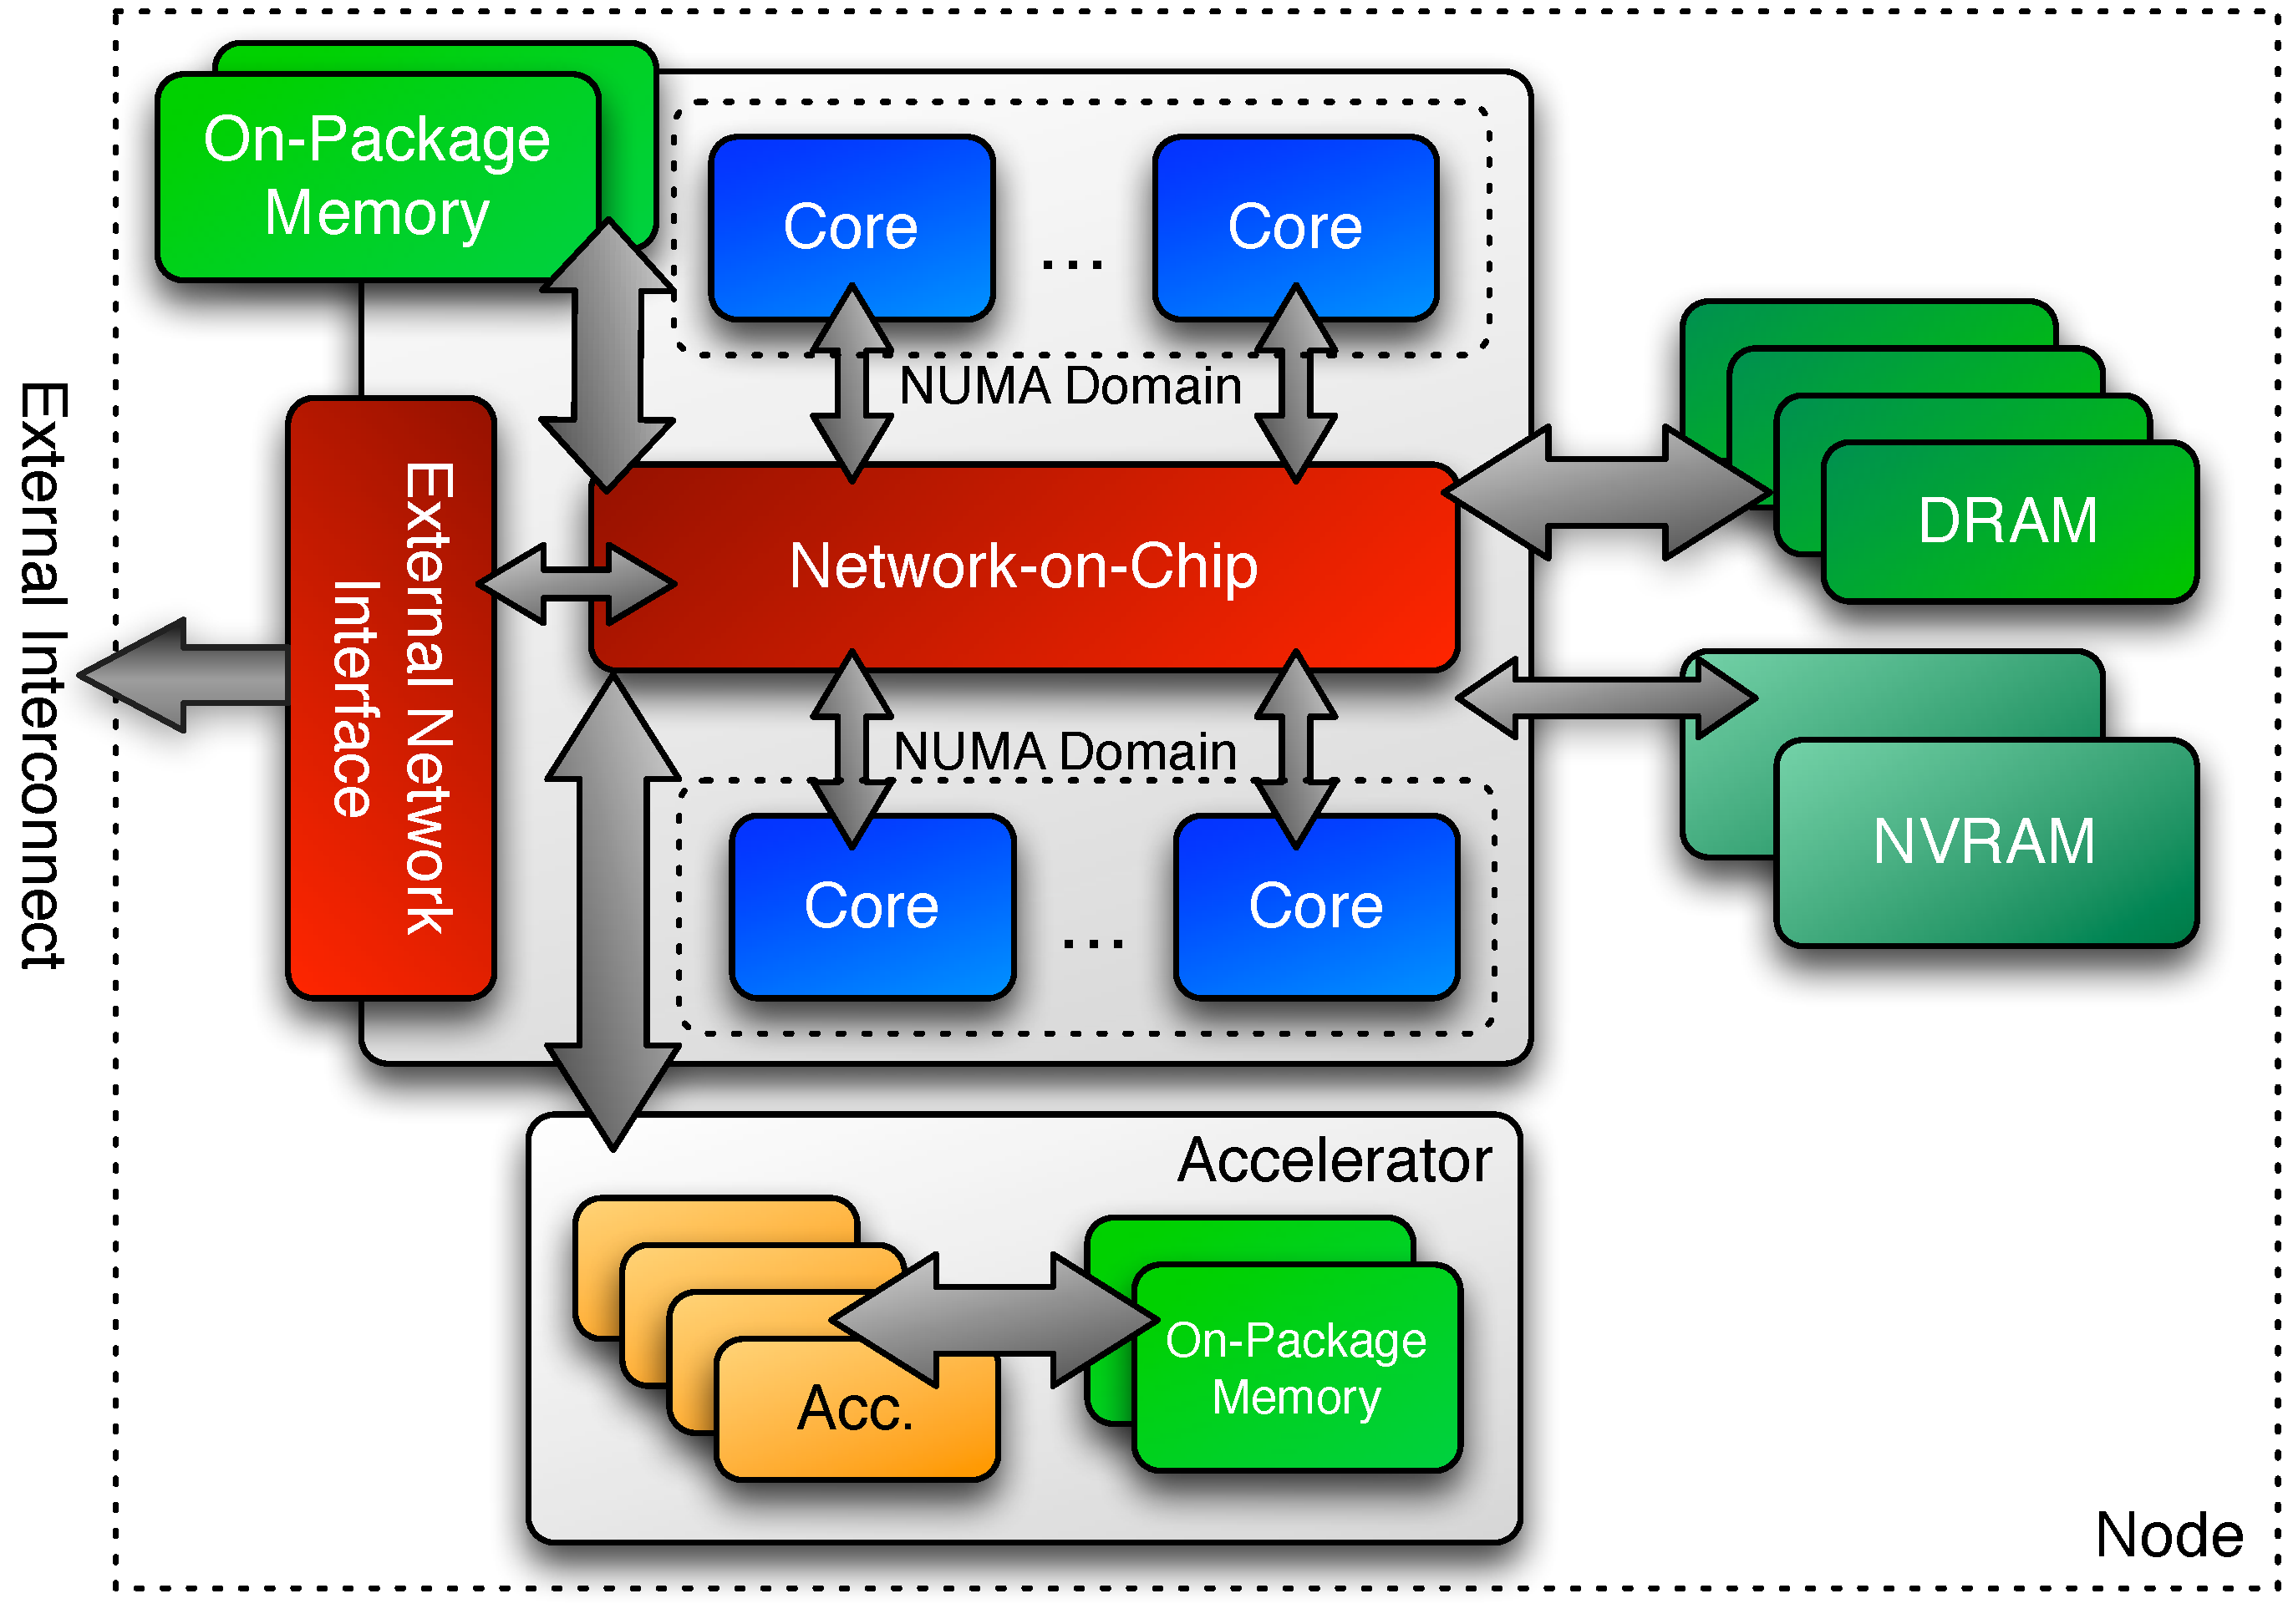
\includegraphics[width=4in]{figures/kokkos-node.pdf}
\caption{Conceptual Model of a Future High Performance Computing Node}
\label{fig:kokkosnode}
\end{center}
\end{figure}

Kokkos assumes an {\em abstract machine model} for the design of
future shared-memory computing architectures. The model (shown in
Figure~\ref{fig:kokkosnode}) assumes that there may be multiple
execution units in a compute node. For a more general discussion
of abstract machine models for Exascale computing the reader should
consult reference~\cite{cal_amm}. In the figure shown here,
we have elected to
show two different types of compute units -- one which represents
multiple latency-optimized cores, similar to contemporary processor
cores, and a second source of compute in the form of an off die
accelerator. Of note is that the processor and accelerator each 
have distinct memories, each with unique performance properties,
that are accessible across the node ({\em i.e.} the memory is
reachable or {\em shared} by all execution units. The specific
layout shown in Figure~\ref{fig:kokkosnode} is an instantiation
of the Kokkos abstract machine model used to describe the potential
for multiple types of compute engines and memories within a single
node. In future systems there may be a range of execution engines
which are used in the node ranging from a single type of core
as in many/multi-core processors found today through to an range
of execution units where many-core processors may be joined to
numerous types of accelerator cores. In order to ensure portability
to the potential range of nodes an abstraction of the
compute engines and available memories are required.

\subsection{Kokkos Execution Spaces}

Kokkos uses the term {\em execution spaces} to describe a logical
grouping of computation units which share an indentical set of
performance properties. An execution space provides a set of 
parallel execution resources which can be utilized by the
programmer using several types of fundamental parallel
operation. For a list of the operations available see
Chapter~\ref{C:Dispatch}.

\subsubsection{Execution Space Instances}

An {\em instance} of an execution space is a specific instantiation
of an execution space to which a programmer can target parallel
work. By means of example, an execution space might be used
to describe a multi-core processor. In this example, the
execution space contains several homogeneous cores which share
some logical grouping. In a program written to the Kokkos model,
an instance of this execution space would be made available
on which parallel kernels could be executed. As a second example,
if we were to add a GPU to the multi-core processor a second
execution space type is available in the system, the 
application programmer would then have two 
execution space instances available to select from. The
important consideration here is that the method of
compiling code for different execution spaces and the
dispatch of kernels to instances is abstracted by the Kokkos
framework allowed application programmers to be free from 
written algorithms in hardware specific languages or
requiring the programmer to understand the restrictions
required for parallel execution in the execution space.

\subsection{Kokkos Memory Spaces}

The multiple types of memory which will become available in future
computing nodes are abstracted by Kokkos through {\em memory
spaces}. Each memory space provides a finite storage capacity
at which data structures can be allocated and accessed. In
order to provide portable allocations and performant access,
Kokkos requires data to be allocated as a $k$-dimensioned array,
where $k$ must be greater than equal to zero (a zero array being
a scalar). Each dimension of the array can be either fixed in
size at compile time or dynamically sized with size resolution
performed during execution.

\subsubsection{Instances of Kokkos Memory Spaces}

In much the same way execution spaces have specific instaniations through
the availablilty of an {\em instance} so do memory spaces. An instance
of a memory space provides a concrete method for the
application programmer to request data storage allocatons. Returning
to the examples provided for execution spaces, the multi-core
processor may have multiple memory spaces available including
on-package memory, slower DRAM and additional a set of non-volatile
memories. The GPU may also provide an additional memory space
through its local on-package memory. The programmer is free
to decide where each data structure may be allocated by requesting
these from the specific instance associated with that memory space.
Kokkos provides the appropriate abstraction of the allocation
routines and any associated data management operations including
releasing the memory and returning it for future use, as well as
copy operations.

\subsubsection{Memory Consistency in Kokkos}

Memory consistency models are a complex topic in and of themselves
and usually rely on complex operations associated with hardware
caches (for more information see reference~\cite{handp_hardware}. 
Kokkos itself does not {\em require} caches to be present
in hardware and so assumes an extremely weak memory consistency
model. In this model, the programmer should not assume any
specific ordering of memory operations being isused by a
kernel. This has the potential to create race conditions between
memory operations if these are not appropriately protected. In
order to provide a guaranteed that memory are completed, Kokkos
provides a {\em fence} operation which forces the compute 
engine to complete all outstanding memory operations before
any new ones can be issued. With appropriate use of fences,
programmers are thereby able to ensure that guarantees can
be made as to when data will {\em definitely} have been 
written to memory.

\subsubsection{Atomic accesses to Memory in Kokkos}


\section{Thread teams}\label{S:Model:Teams}

Kokkos supports multiple levels of parallelism.
In particular, it groups threads into \emph{teams}.
A \emph{thread team} is a collection of one or more parallel ``threads'' of execution.
Kokkos allows an arbitrary number of teams -- the \emph{league size}.
Hardware constrains the number of threads in a team -- the \emph{team size}.

Threads in a team can synchronize -- they have a ``barrier'' primitive -- 
and share a ``scratch pad'' memory which they may use for temporary storage.
Scratch pad memory exists only during parallel operations;
allocations in it do not persist across kernels.
Teams themselves may run in any order,
and may not necessarily run all in parallel.
For example, if the user asks for $T$ teams,
the hardware may choose to run them one after another in sequence,
or in groups of up to $G$ teams at a time in parallel.

Users may \emph{nest} parallel operations.
Teams may perform one parallel operation (for, reduce, or scan),
and threads within each team may perform another, possibly different parallel operation.
Different teams may do entirely different things.
For example, all the threads in one team may execute a \lstinline!parallel_for!,
and all the threads in a different team may execute a \lstinline!parallel_scan!.
Different threads within a team may also do different things.
However, performance may vary if threads in a team ``diverge'' in their behavior
(e.g., take different sides of a branch).
Chapter \ref{C:Hierarchical} shows how the C++ implementation of Kokkos exposes thread teams.

NVIDIA's CUDA programming model inspired Kokkos' thread team model.
The scratch pad memory corresponds with CUDA's per-team ``shared memory.''
The ``league / team'' vocabulary comes from OpenMP 4.0,
and has many aspects in common with our thread team model.
We have found that programming to this model results in good performance,
even on computer architectures which only implement parts of the full model.
For example, most multicore processors in common use for high-performance computing lack ``scratch pad'' hardware.
However, if users request a scratch pad size that fits comfortably in the largest cache shared by the threads in a team,
programming as if a scratch pad exists forces users to address locality in their algorithms.
This also reflects the common experience that rewriting a code for more restrictive hardware,
then porting the code \emph{back} to conventional hardware,
tends to improve performance relative to an unoptimized code.

\section{Program execution}\label{S:Model:Exec}

It is tempting to try to define formally what it means for a processor to execute code.
None of us authors have a background in logic or what computer scientists call ``formal methods,''
so our attempt might not go very far!
We will stick with informal definitions and rely on Kokkos' C++ implementation
as an existence proof that the definitions make sense.

Kokkos lets users tell execution spaces to execute parallel operations.
These include parallel for, reduce, and scan (see Chapter \ref{C:Dispatch})
as well as View allocation and initialization (see Chapter \ref{C:View}).
We name the class of all such operations \emph{parallel dispatch}.

From our perspective, there are three kinds of code:
\begin{enumerate}
\item Code executing inside of a Kokkos parallel operation
\item Code outside of a Kokkos parallel operation that asks Kokkos to
  do something (e.g., parallel dispatch itself)
\item Code that has nothing to do with Kokkos
\end{enumerate}
The first category is the most restrictive.
Section \ref{S:Model:Teams} above explains restrictions on inter-team synchronization.
In general, we limit the ability of Kokkos-parallel code to invoke Kokkos operations
(other than for nested parallelism; 
see Section \ref{S:Model:Teams} above and Chapter \ref{C:Hierarchical}).
We also forbid dynamic memory allocation (other than from the team's scratch pad) in parallel operations.
Whether Kokkos-parallel code may invoke operating system routines or third-party libraries
depends on the execution and memory spaces being used.
Regardless, restrictions on inter-team synchronization have implications for things like filesystem access.

\emph{Kokkos threads are for computing in parallel,}
not for overlapping I/O and computation,
and not for making graphical user interfaces responsive.
Use other kinds of threads (e.g., operating system threads) for the latter two purposes.
You may be able to mix Kokkos' parallelism with other kinds of threads;
see Section \ref{SS:Model:Exec:ThreadSafety}.
Kokkos' developers are also working on a task parallelism model
that will work with Kokkos' existing data-parallel constructs.

\subsection{Reproducible reductions and scans}\label{SS:Model:Exec:Repro}

Kokkos promises \emph{nothing} about the order in which the iterations of a parallel loop occur.
However, it \emph{does} promise that if you execute the same parallel reduction or scan,
using the same hardware resources and run-time settings,
then you will get the same results each time you run the operation.
``Same results'' even means ``with respect to floating-point rounding error.''

\subsection{Asynchronous parallel dispatch}\label{SS:Model:Exec:Async}

This concerns the second category of code, that calls Kokkos operations.
In Kokkos, parallel dispatch executes \emph{asynchronously}.  
This means that it may return ``early,'' before it has actually completed.
Nevertheless, it executes \emph{in sequence} with respect to other Kokkos operations on the same execution or memory space.
This matters for things like timing.
For example, a \lstinline!parallel_for! may return ``right away,''
so if you want to measure how long it takes,
you must first call \lstinline!fence()! on that execution space.
This forces all functors to complete before \lstinline!fence()! returns.

\subsection{Thread safety?}\label{SS:Model:Exec:ThreadSafety}

Users may wonder about ``thread safety,'' that is,
whether multiple operating system threads may safely call into Kokkos concurrently.
Kokkos' thread safety depends on both its implementation, 
and on the execution and memory spaces that the implementation uses.
The C++ implementation has made great progress towards (non-Kokkos) thread safety of View memory management.
For now, however, the most portable approach is for only one (non-Kokkos) thread of execution to control Kokkos.
Also, be aware that operating system threads might interfere with Kokkos' performance,
depending on the execution space that you use.

Thread safety with respect to Kokkos' threads is a different matter.
View (see Chapter \ref{C:View}) promises safety of its memory management.
That is, you may safely access Views inside of Kokkos' parallel operations.
Kokkos provides some synchronization constructs as well; see the following section.

\section{Memory consistency}\label{S:Model:Consistency}

A \emph{memory consistency model} describes the behavior of a memory space $M$,
with respect to multiple threads running in an execution space $E$
that access the same data in $M$ concurrently.
One may also encounter this idea as the phrase ``cache coherency.''
We prefer ``memory consistency,'' because Kokkos does not require caches.
Consistency models are a complicated subject which we cannot cover in sufficient detail here.
We encourage readers to refer to standard computer hardware textbooks,
like ``Computer Architecture: A Quantitative Approach'' (Hennessy and Patterson, 2011).

Kokkos imposes a very weak consistency model across an entire execution space.
For example, it does \emph{not} assume sequential consistency.
Much like MPI 3 one-sided communication
or other partitioned global address space (PGAS) programming models,
Kokkos requires an execution space to issue a \emph{memory fence}
to a given memory space, 
in order to bring that memory space into a consistent state.
The fence forces completion of all outstanding memory writes,
and reorders all loads to occur after all those writes complete.

\subsection{Atomic updates}\label{SS:Model:Consistency:Atomic}

Some execution spaces may implement \emph{atomic updates} with respect to some memory spaces.
An atomic update runs on an execution space, and changes a word of data in a memory space.
The atomic update behaves atomically with respect to other atomic updates happening concurrently by that execution space on that memory space.
``Behaves atomically'' means that all of the atomic updates will complete,
and the word of data will be changed in a way that respects some order of those update operations.
Kokkos does not promise any particular order.
Furthermore, for a nonatomic memory read or write to ``see'' the results of atomic updates,
the execution space must first execute a \lstinline!fence()! operation to that memory space.
